\documentclass[../../main.tex]{subfiles}

\begin{document}

\section{Datasets}

\subsection{Gaussian Process}

The 2D Gaussian Process is the natural extension of the 1D Gaussian Process described in \autoref{sec:1d-gp-dataset} where we use the squared exponential kernel. We continue to use the same range of lengthscale across both input dimensions as the 1D Gaussian Process. 

The following plots show some samples from the GP dataset.

\todo{Add plots of GP dataset}


\subsection{Sawtooth}

The 2D Sawtooth dataset is the natural extension of the 1D Sawtooth dataset described in \autoref{sec:1d-sawtooth-dataset}. We continue to use the same period $T$ and noise $n$ across both input dimensions as the 1D Sawtooth dataset.

The following plots show some samples from the Sawtooth dataset.

\todo{Add plots of Sawtooth dataset}

\subsection{Restricted Sawtooth}

By accident when generating the 2D Sawtooth dataset, we ended up restricted the `direction of travel' of the sawtooth function to the line of $x_1 = x_2$ or $x_1 = -x_2$. This was not intentional but when training both models on this dataset, we found very interesting results. As the models only learn a subset of the `full sawtooth' function, we can see how well the models can generalize to samples from the full sawtooth function.

The following plots show some samples from the Restricted Sawtooth dataset.

\section{Post or Pre Relative Attention Function}

\todo{Highlight MLP}

In our original formulation of the TETNP (\autoref{sec:tetnp}) we pass the matrix of differences ($\bm{\Delta}$) between $x$ values through a function $F$ to apply non-linearities then add it to the dot product attention \autoref{eq:relative-attention}, whilst this performs well we can also consider applying this non-linearity after combining the dot product attention and the relative attention, this method is called the `Post Relative Attention Function'. 

\begin{align}
	\text{Attention}(\bm{Q}, \bm{K}, \bm{V}, \bm{X}) &= \text{softmax}\left(\bm{E} \right) \bm{V}
\end{align}
\begin{align}
	\text{Pre:} \quad \bm{E_{ij}} &= \bm{D_{ij}}+ \text{MLP}(\bm{\Delta_{ij}})\\
    \text{Post:} \quad \bm{E_{ij}} &= \text{MLP}(\texttt{cat}[ \bm{D_{ij}}, \bm{\Delta_{ij}}])
\end{align}
Where 
\begin{align}
     \bm{D_{ij}} = \bm{q_i} \cdot \bm{k_j}  /\sqrt{d_k} \quad \quad    \bm{\Delta_{ij}} = \bm{x_i} - \bm{x_j}
\end{align}


We will investigate the performance of the TETNP with the `Post Relative Attention Function' compared to the original `Pre Relative Attention Function'. We choose to use the Sawtooth dataset as it is more difficult to learn than the Gaussian Process dataset and will show the differences between the two models more clearly. 


% Figure ./post-pre-kernel.pdf
\begin{figure}[H]
    \centering
    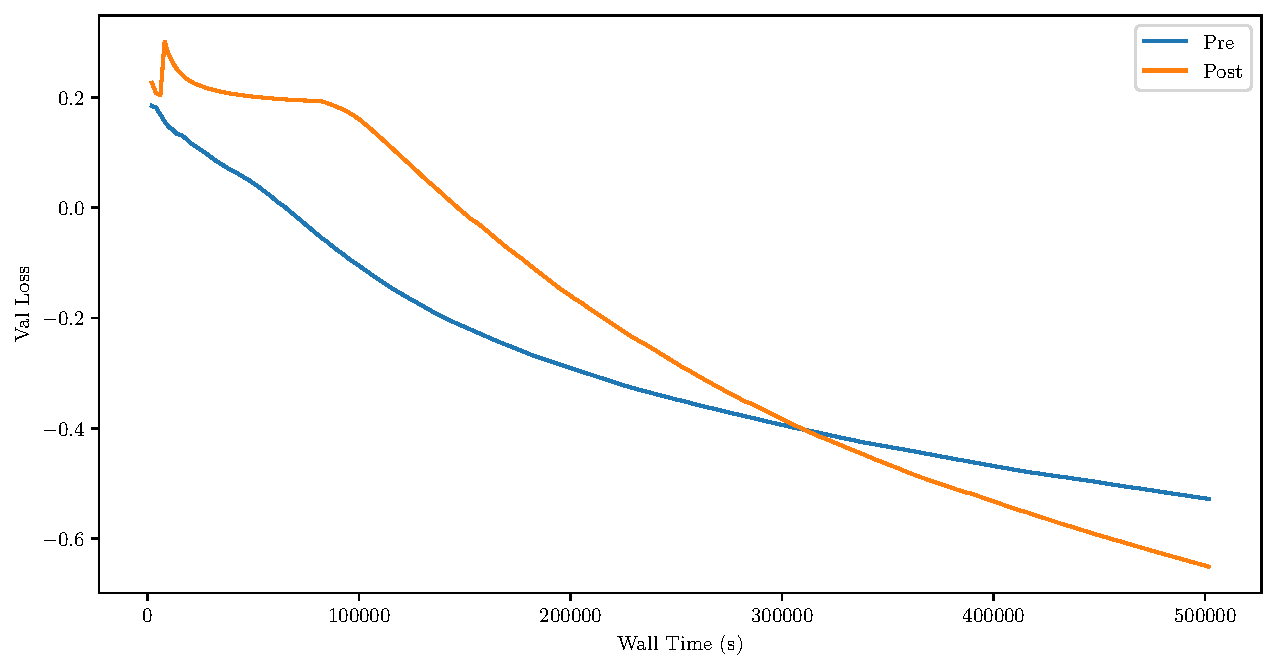
\includegraphics[width=0.8\linewidth]{./fig/post-pre-kernel.pdf}
    \caption{Validation Loss of TETNP with the `Post Relative Attention Function' and `Pre Relative Attention Function' on the 2D Sawtooth Dataset. Lower validation loss is better.}
    \label{fig:post-pre-kernel}
\end{figure}


The results show that the TETNP with the `Post Relative Attention Function' outperforms the TETNP with the `Pre Relative Attention Function' by quite a large margin. Trivially this makes a lot of sense as the Post function can further refine the dot product attention through the MLP whilst in the `Pre' function the MLP is \emph{only} applied to the $\bm{\Delta}$ matrix. The computational complexity of these two functions are not too different as the MLP are small and applied to the same size matrices. 


\section{ConvNP vs TETNP}

We have discovered in the 1D section that the TETNP outperforms the vanilla TNP in all cases, hence for the 2D experiments we will only compare the ConvNP to the TETNP. When performing our experiments we will use models which are both 1 million parameters in size, to ensure a fair comparison.

\subsection{Gaussian Process}

As mentioned previously, the Gaussian Process dataset is not very difficult to learn and the ConvNP and TETNP both perform very well on this dataset with the TETNP outperforming the ConvNP by a small margin as shown in \autoref{tab:gp-2d-val-doss}.

\begin{table}[ht]
    \centering
    \begin{tabular}{lc}
        \toprule
        Model  & Validation Loss \\
        \midrule
        ConvNP & 1.168           \\
        TETNP  & 1.134           \\
        \bottomrule
    \end{tabular}
    \caption{Validation Loss of ConvNP and TETNP on the 2D Gaussian Process dataset after training for 3 hours using 1 million parameters models and 64 context points. Lower is better.}
    \label{tab:gp-2d-val-doss}
\end{table}

Observing the samples from the ConvNP and TETNP for low frequency \autoref{fig:low-freq-2d-gps} and high frequency functions \autoref{fig:high-freq-2d-gps}, we can see both models are able to generate very similar predictions to the ground truth GP. The TETNP performs slightly better than the ConvNP in the low frequency case, but the ConvNP performs better in the high frequency case for these samples. However overall the TETNP performs better than the ConvNP on the Gaussian Process dataset.

\begin{figure}[H]
	\centering
	\subfloat[ConvNP (top plot is the model prediction and bottom is the ground truth GP)]{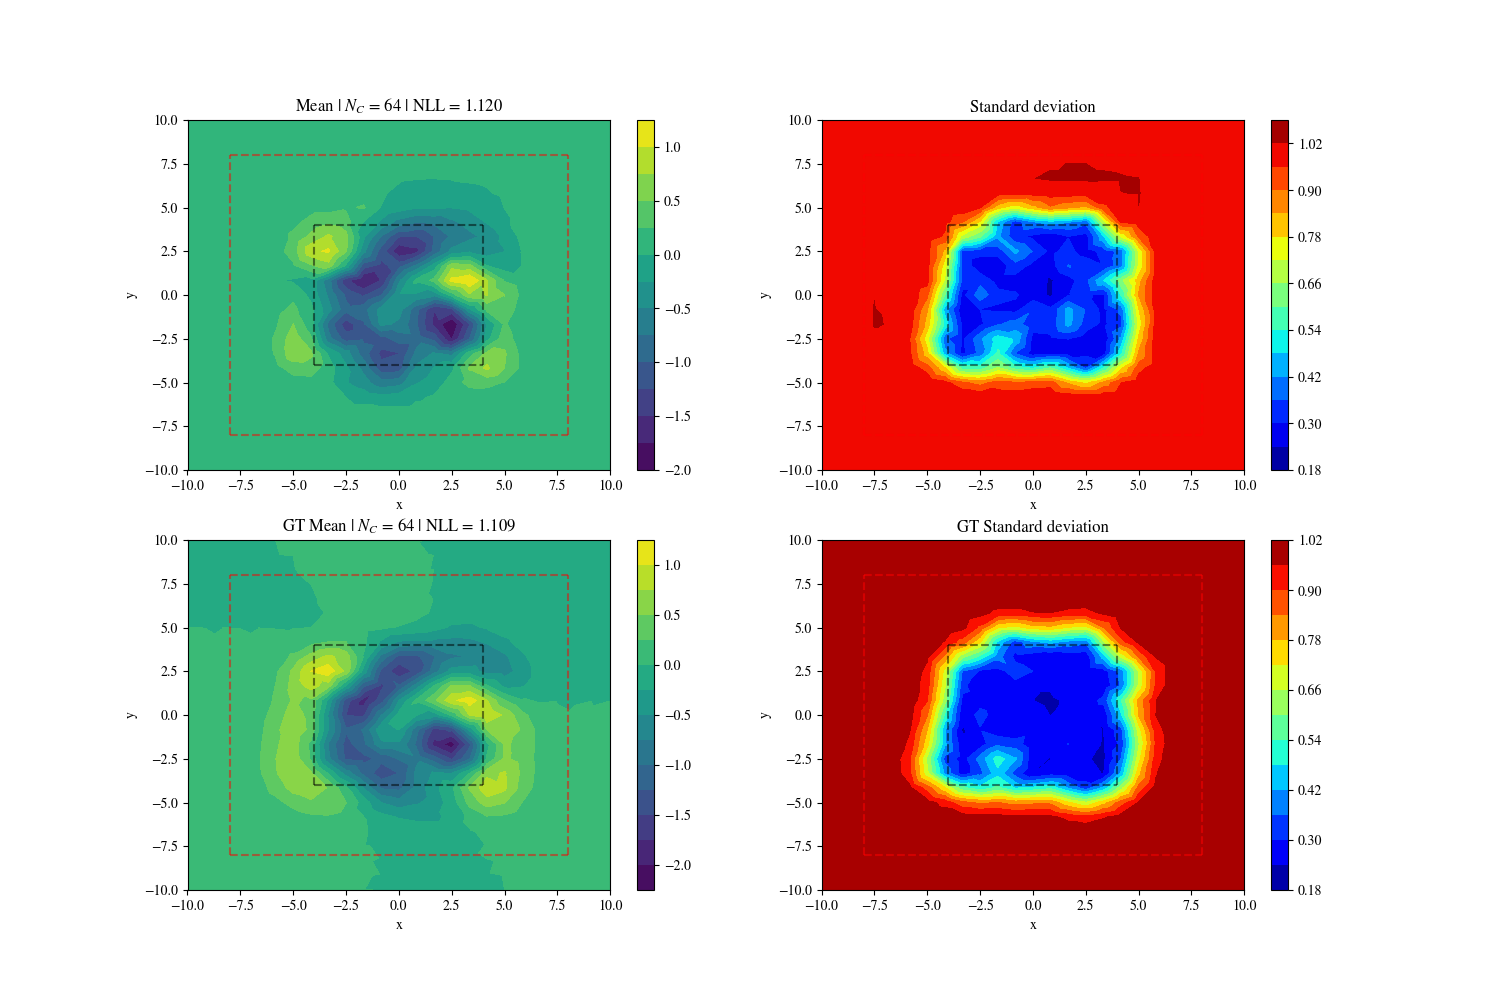
\includegraphics[width=0.8\linewidth]{./fig/gp/conv-gp-2d.png}}\\
	\subfloat[TETNP (top plot is the model prediction and bottom is the ground truth GP)]{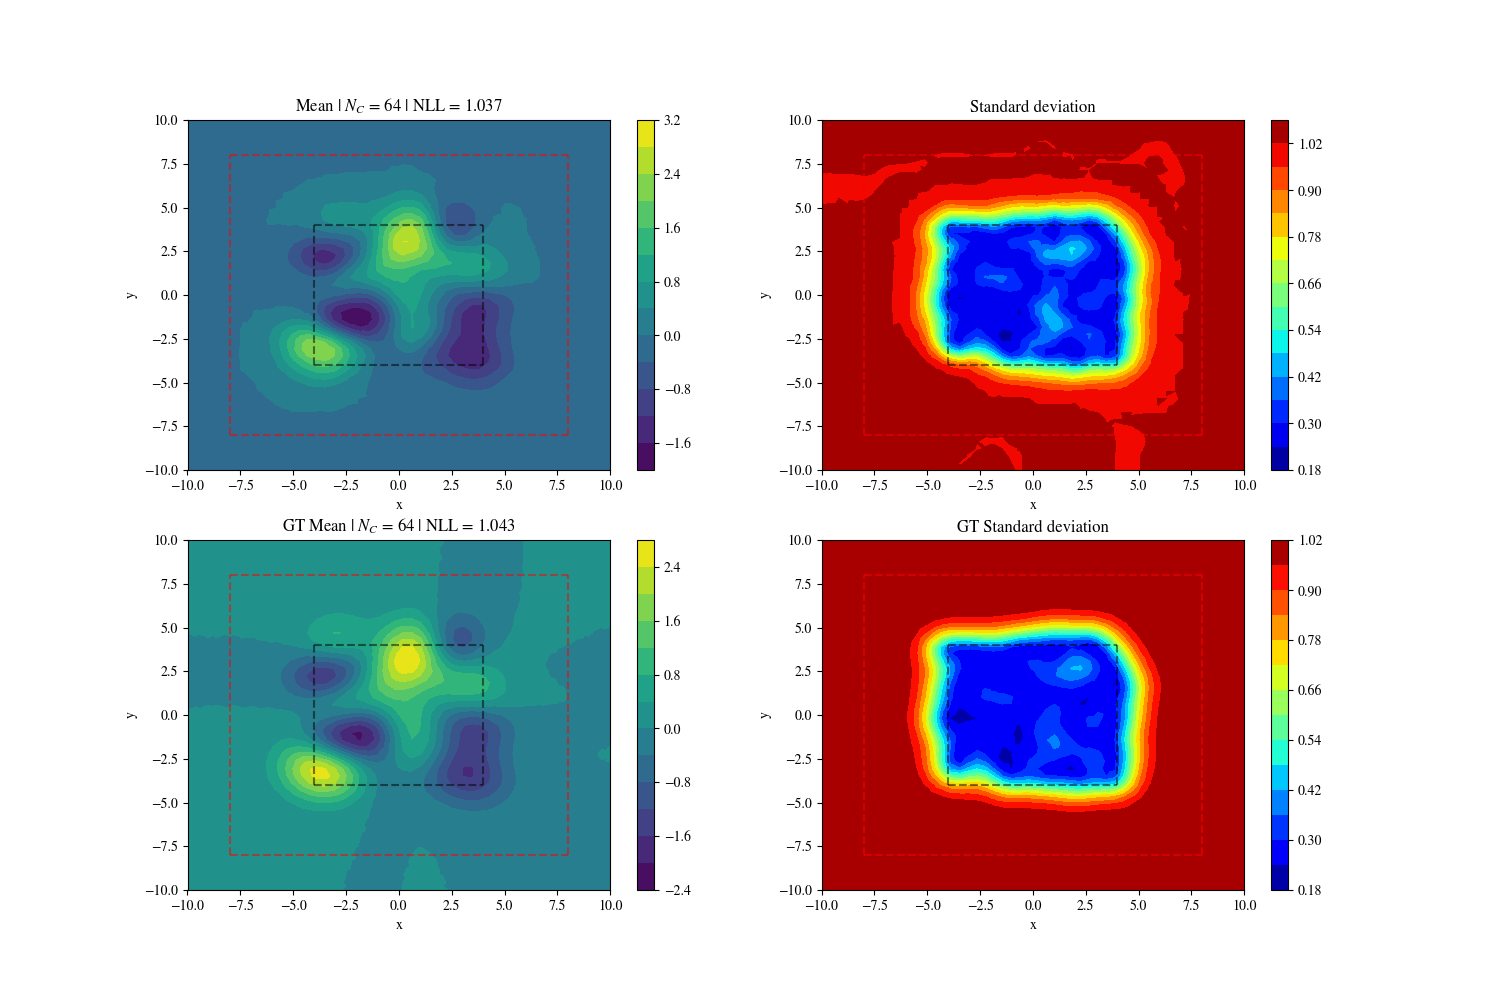
\includegraphics[width=0.8\linewidth]{./fig/gp/tetnp-gp-2d.png}}
	\caption{Samples from ConvNP and TETNP on a low frequency 2D Gaussian Process.}
	\label{fig:low-freq-2d-gps}
\end{figure}

\begin{figure}[H]
	\centering
	\subfloat[ConvNP (top plot is the model prediction and bottom is the ground truth GP)]{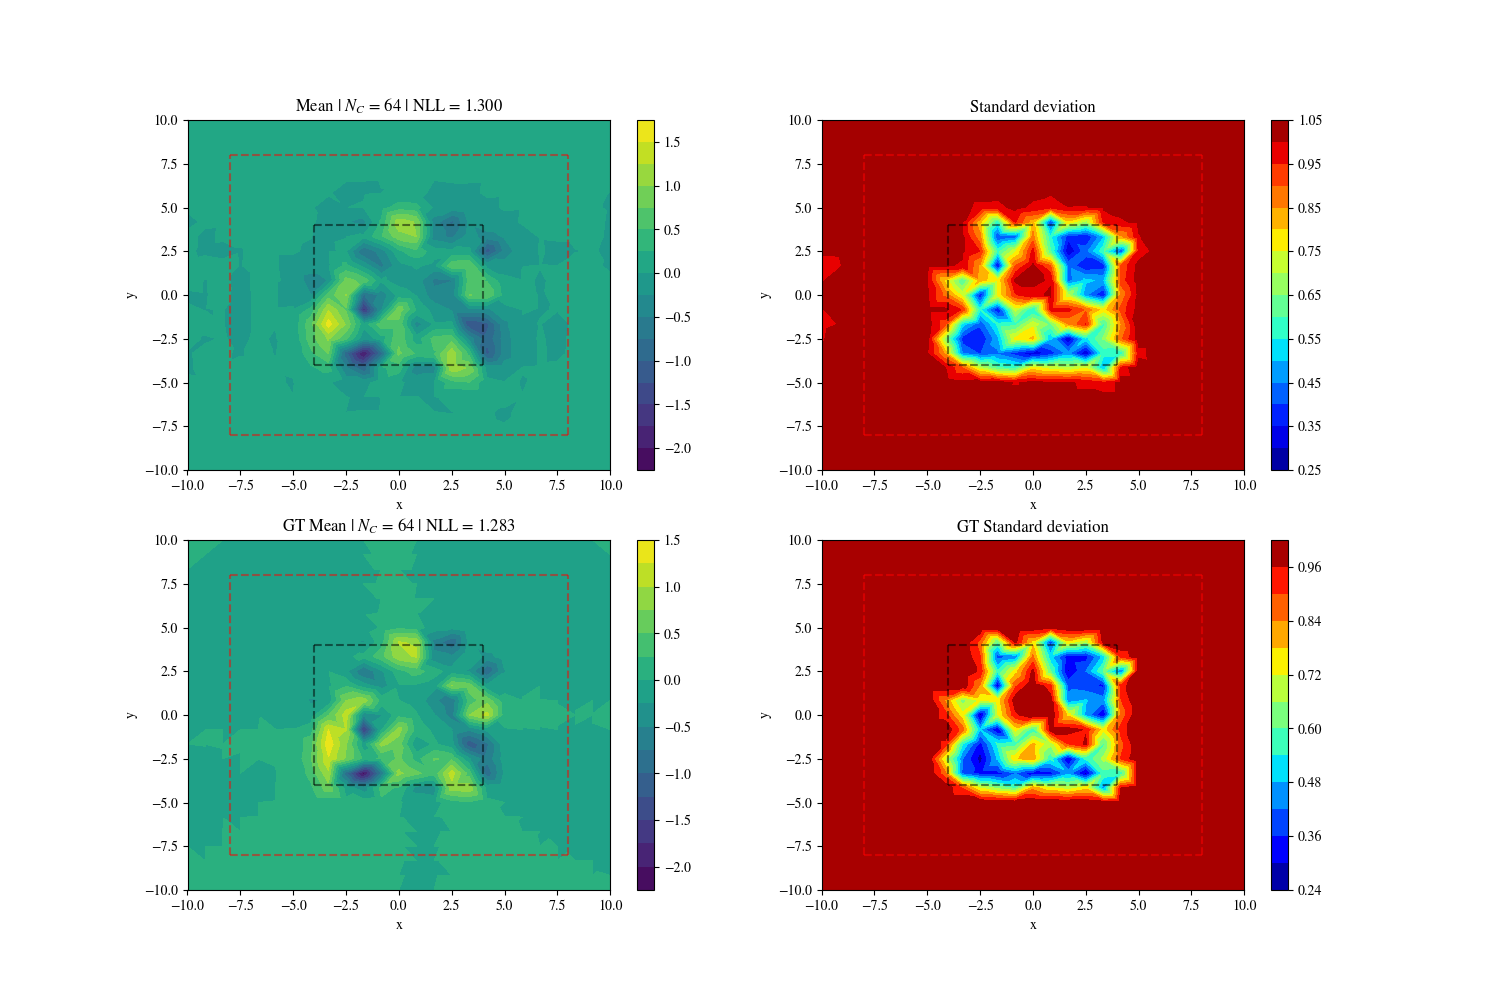
\includegraphics[width=0.8\linewidth]{./fig/gp/conv-gp-2d-2.png}}\\
	\subfloat[TETNP (top plot is the model prediction and bottom is the ground truth GP)]{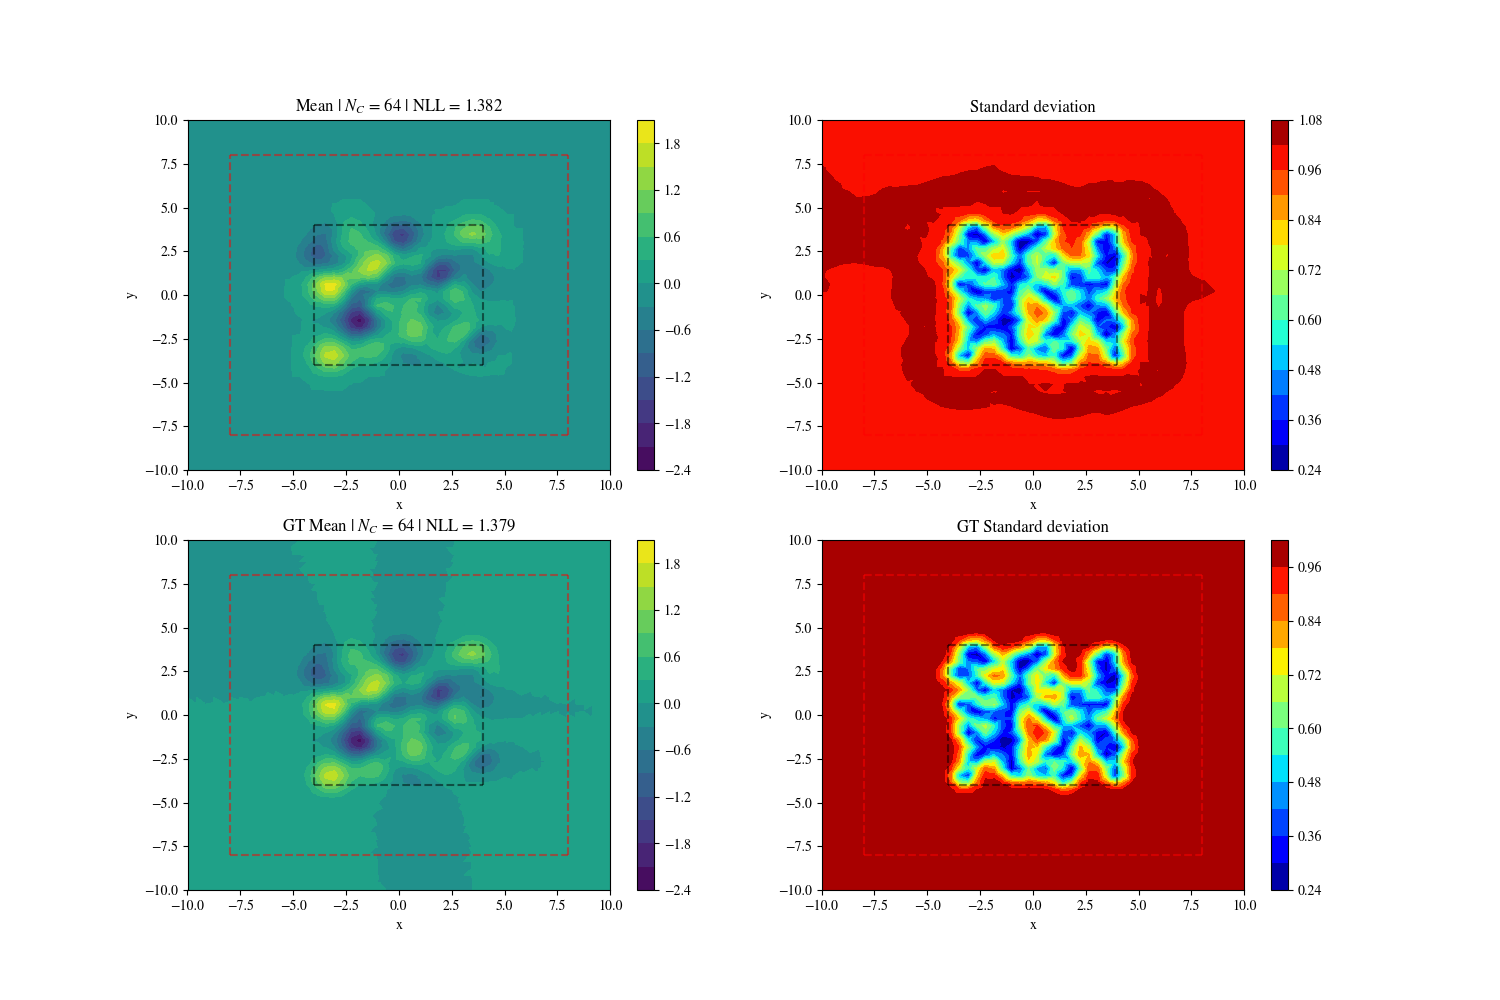
\includegraphics[width=0.8\linewidth]{./fig/gp/tetnp-gp-2d-2.png}}
	\caption{Samples from ConvNP and TETNP on a high frequency 2D Gaussian Process.}
	\label{fig:high-freq-2d-gps}
\end{figure}

\subsection{Restricted Sawtooth and Rotational Equivariance}

As previously stated the restricted sawtooth dataset is a subset of the full sawtooth dataset which restricts the `direction of travel' of the sawtooth function to the line of $x_1 = x_2$ or $x_1 = -x_2$. By training both models on this dataset we can see how well the models can generalize.
% Figure ./fig/res-saw/te.png and ./fig/res-saw/conv.png

\begin{figure}[H]
    \centering
    \subfloat[TETNP]{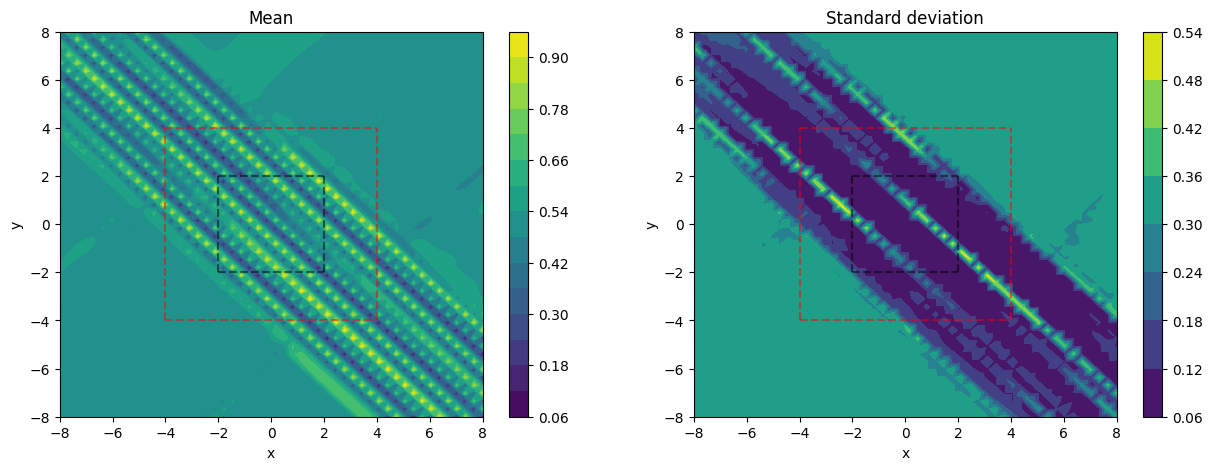
\includegraphics[width=0.8\linewidth]{./fig/res-saw/te.png}}\\
    \subfloat[ConvNP]{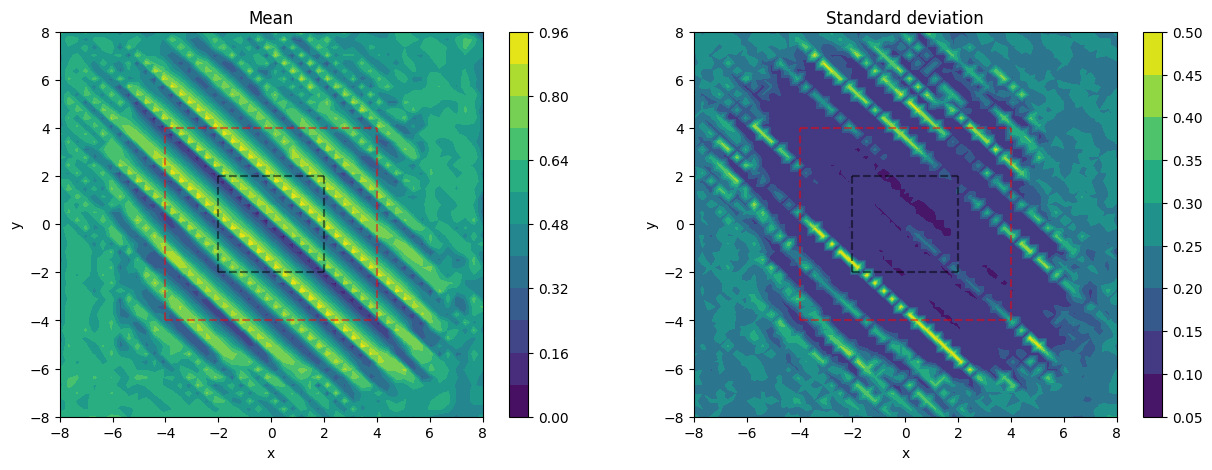
\includegraphics[width=0.8\linewidth]{./fig/res-saw/conv.png}}
    \caption{Samples from TETNP and ConvNP on the Restricted Sawtooth dataset. The region inside the black dotted box is the region the models were trained on and the region outside the black dotted box is the region the models were not trained on.}
    \label{fig:res-saw-preds}
\end{figure}

\autoref{fig:res-saw-preds} shows that the ConvNP performs excellently on this dataset, which is expected as CNNs have filters which learn features and patterns in the data explicitly, thus performs well on extrapolation tasks (outside the black dotted box region). The TETNP on the other hand struggles to generalize fully within the target region (red dotted box) and outside the target region. Instead, it learns to extrapolate the sawtooth along one axis, but not the other. This clearly highlights a limitation of the Transformer architecture which has very little interpretability hence producing weird results.

\emph{Is this TETNP able to generalize to the full sawtooth dataset?} To answer this question we will simply run the TETNP on a rotated version of the restricted sawtooth dataset which is the full sawtooth dataset.



% Figure ./fig/res-saw/no-re.png

\begin{figure}[H]
    \centering
    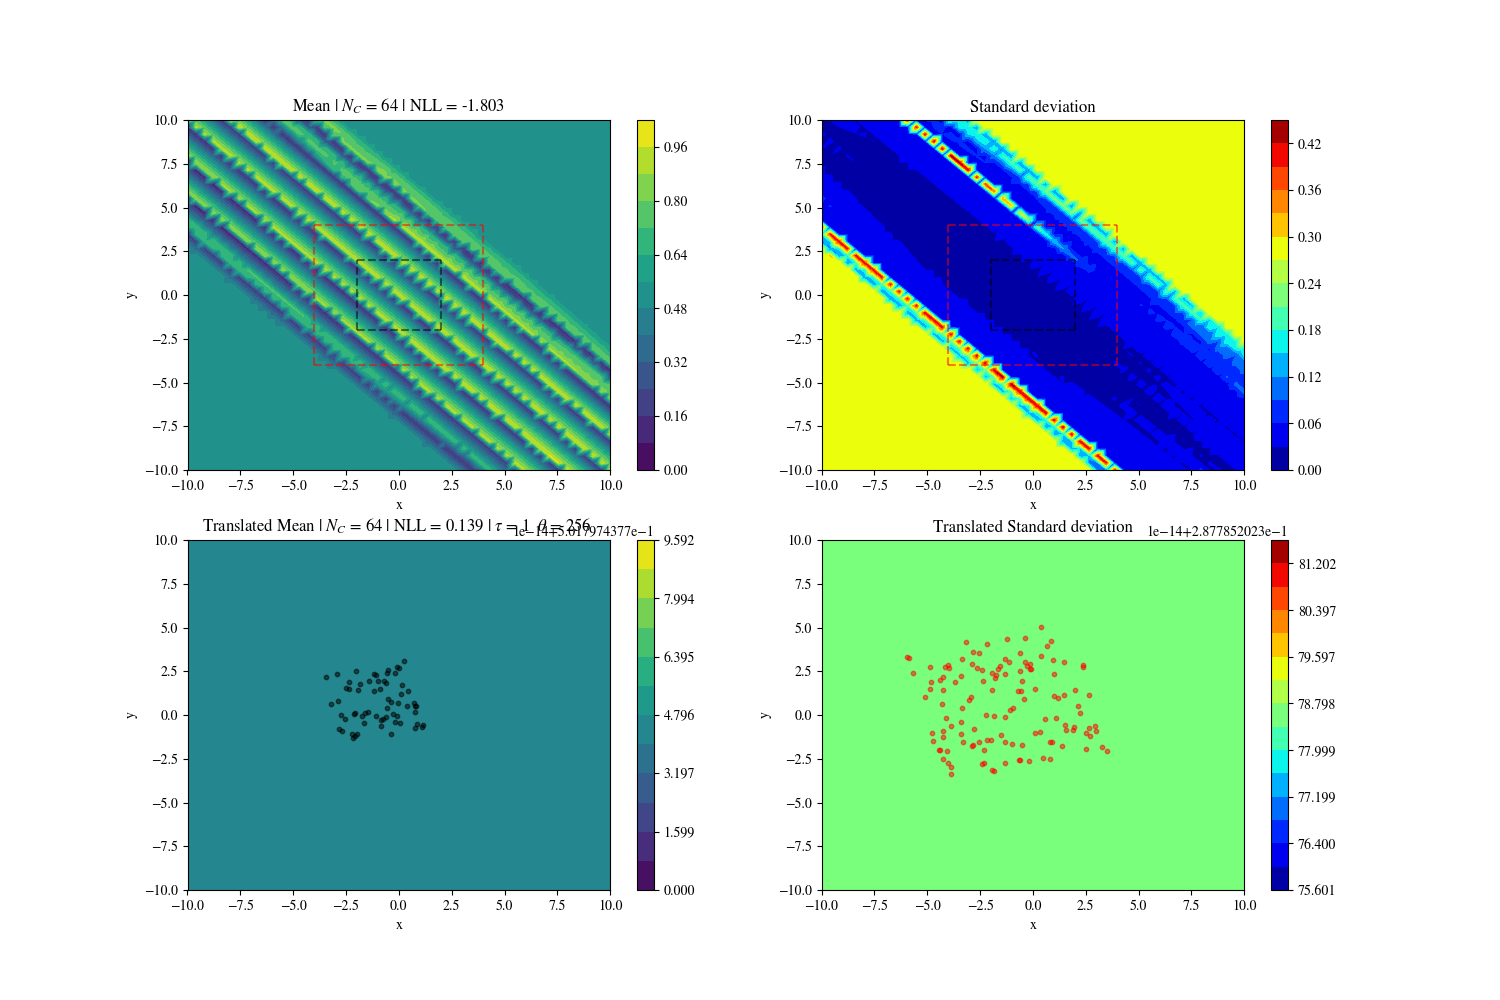
\includegraphics[width=0.8\linewidth]{./fig/res-saw/no-re.png}
    \caption{Samples from TETNP on the full Sawtooth dataset. The top plot is the model prediction on the restricted sawtooth dataset and the bottom plot is the model prediction on the full sawtooth dataset which is a rotated version of the restricted sawtooth dataset.
    The region inside the black dotted box is the region the model was trained on and the region outside the black dotted box is the region the model was not trained on.}
    \label{fig:no-re-saw-preds}
\end{figure}

In \autoref{fig:no-re-saw-preds} we explicitly reduced the target and context region size to allow for the TETNP to cover the full target region. The bottom plot shows the predictions when we rotate the context points by 256 degrees, clearly the TETNP completely fails, it just predicts a constant mean and standard deviation. \emph{Could introducing rotational equivariance to the TETNP help it generalize to the full sawtooth dataset?}

\subsubsection{Rotational Equivariance}

To introduce rotational equivariance is fairly simple, in our formulation of the Translation Equivariance Attention, we use a matrix $\bm{\Delta}$ which is the difference between the $\bm{x}$ values of all the data points.

\begin{align}
    \text{Not RE}: \quad &\bm{\Delta}_{ij} = \bm{x}_i - \bm{x}_j\\
    \text{RE}: \quad &\bm{\Delta}_{ij} = \|\bm{x}_i - \bm{x}_j\|_2
\end{align}

To introduce rotational equivariance we can simply take the L2 norm of the $\bm{\Delta}$ matrix which will give us the distance between all the data points. Distances are invariant to rotation, hence the TETNP should be rotationally equivariant. Using this new $\bm{\Delta}$ matrix we can train the TETNP on the restricted sawtooth dataset and see if it can generalize to the full sawtooth dataset.

% Figure ./fig/res-saw/re.png

\begin{figure}[H]
    \centering
    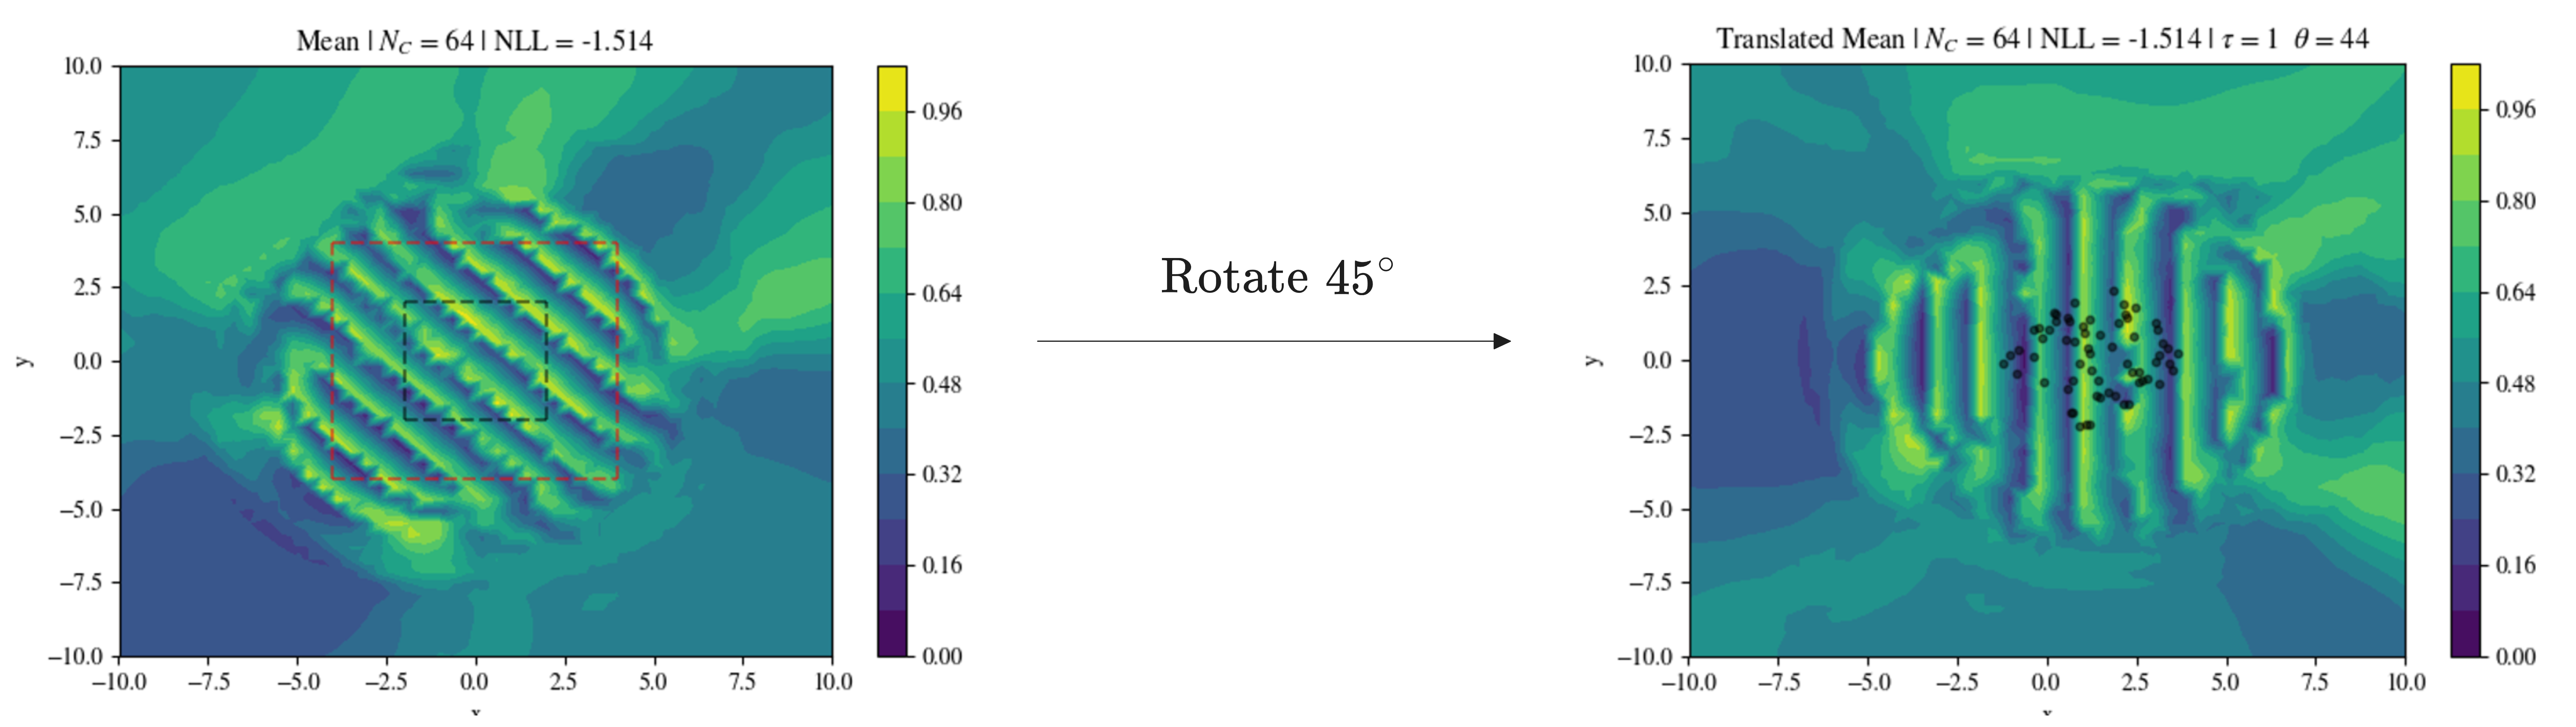
\includegraphics[width=0.8\linewidth]{./fig/res-saw/re.png}
    \caption{Samples from TETNP on the full Sawtooth dataset with Rotational 
    The region inside the black dotted box is the region the model was trained on and the region outside the black dotted box is the region the model was not trained on.}
    \label{fig:re-saw-preds}
\end{figure}

\autoref{fig:re-saw-preds} demonstrates a massive improvement in the TETNP's ability to generalize to the full sawtooth dataset. Hence, we can conclude that RE is beneficial for the case when the inherent structure of the data is rotationally invariant. This illustrates a massive benefit of the Transformer architecture, as \textbf{it is very easy to introduce inductive biases to the Transformer model}, which is not the case for CNNs.

However, as we will see in the next section, if the data given to the model contains samples from many directions, the model will learn to be RE.

\subsection{Full Sawtooth}

The full sawtooth dataset is the full sawtooth function which is not restricted to any direction of travel. We observe that the TETNP is able to generalize to the full sawtooth dataset without the need for rotational equivariance \autoref{fig:full-saw-preds}. 

% Figure ./fig/saw/tetnp.png and ./fig/saw/tetnp2.png and ./fig/saw/tetnp3.png

\begin{figure}[H]
    \centering
    \subfloat[]{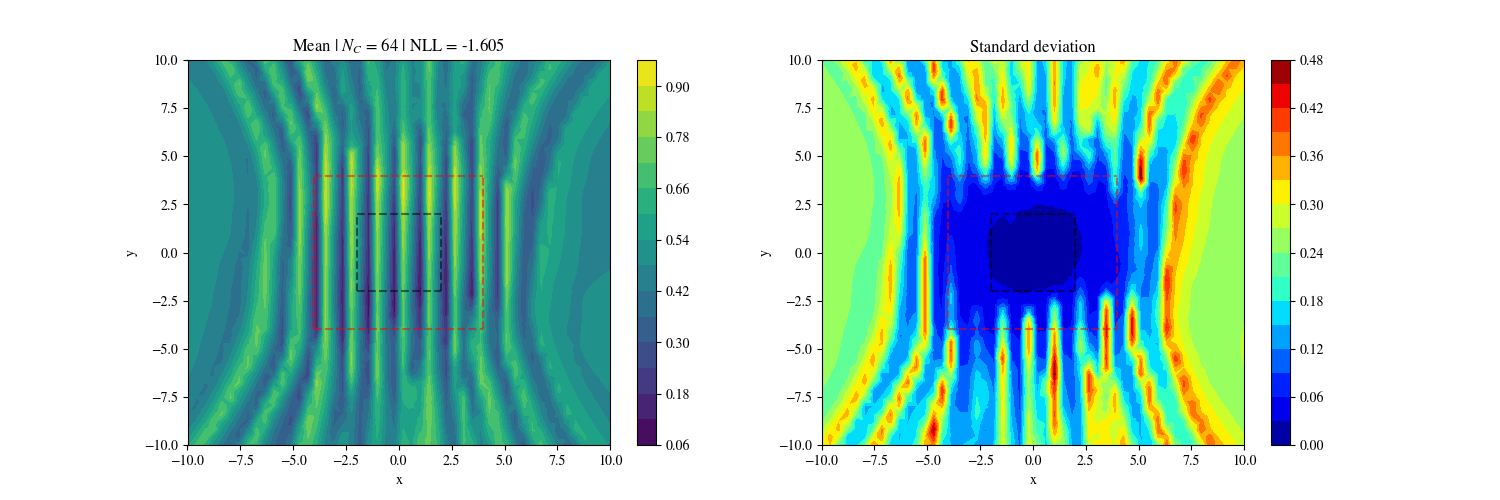
\includegraphics[width=0.8\linewidth]{./fig/saw/tetnp.png}}\\
    \subfloat[]{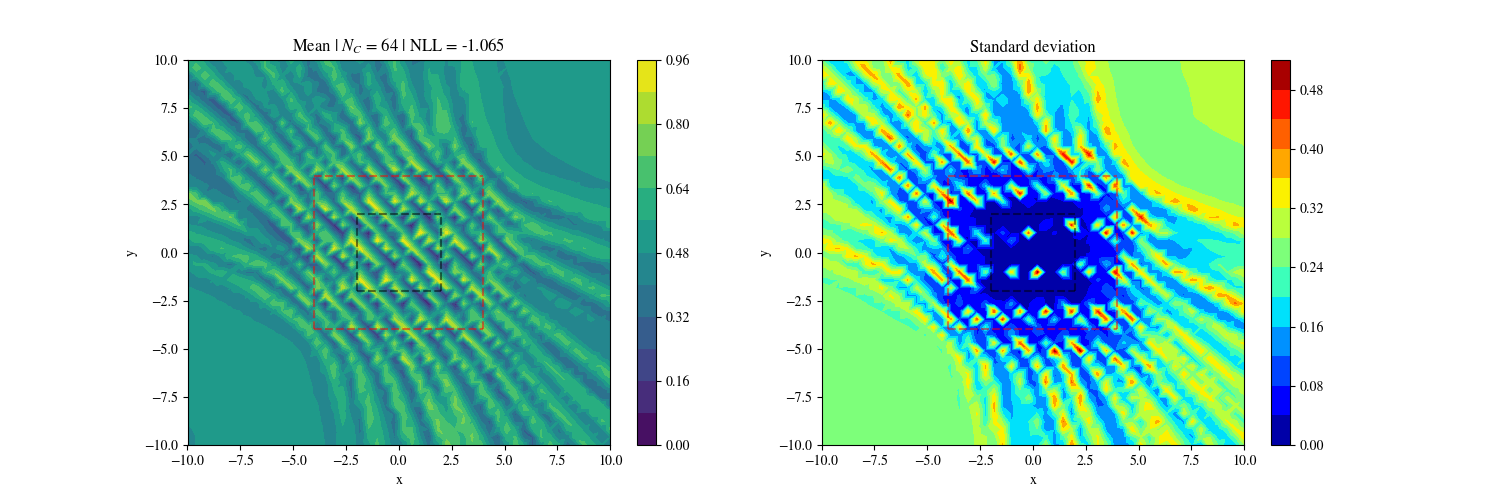
\includegraphics[width=0.8\linewidth]{./fig/saw/tetnp-2.png}}\\
    \subfloat[]{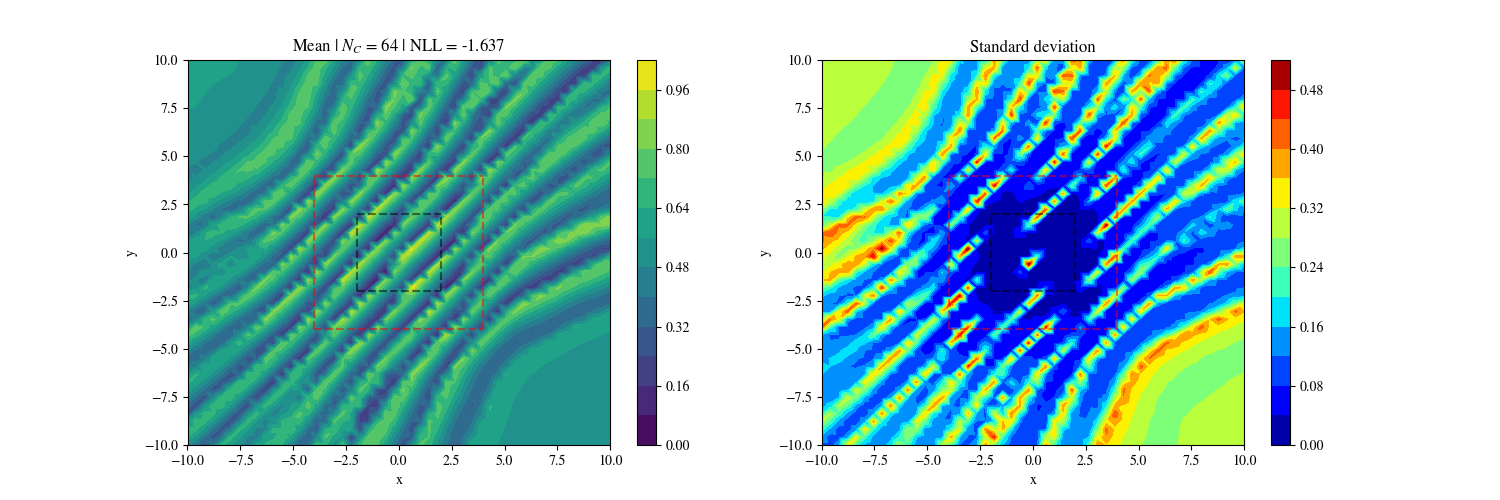
\includegraphics[width=0.8\linewidth]{./fig/saw/tetnp-3.png}}
    \caption{Samples from TETNP on the full Sawtooth dataset. The region inside the black dotted box is the region the model was trained on and the region outside the black dotted box is the region the model was not trained on.}
    \label{fig:full-saw-preds}
\end{figure}

% Compared to the ConvNP the TETNP does indeed perform better in terms of validation loss.

\todo{GET PLOTS OF CONVNP ON FULL SAWTOOTH AND COMPARE RESULTS!!!!!!!!!!!!\\!\\!\\!\\!}

\begin{table}[]
    \begin{tabular}{@{}llll@{}}
    \toprule
    $N_c$ & $N_t$ & ConvNP Memory (MB) & TETNP Memory (MB) \\ \midrule
    10    & 10    & 24                 & 13                \\
    100   & 10    & 29                 & 23                \\
    1000  & 10    & 257                & 984               \\
    5000  & 10    & 1273               & 24082             \\ \midrule
    10    & 1000  & 268                & 26                \\
    100   & 1000  & 268                & 113               \\
    1000  & 1000  & 268                & 985               \\
    5000  & 1000  & 1273               & 24083             \\ \bottomrule
    \end{tabular}
    \end{table}


\section{Computational Complexity}

\todo{Run the code for this \\!\\!\\!\\!}

\ifSubfilesClassLoaded{%
    \printbibliography{}
}{} 


\end{document}